\chapter{\color{blue}Experimentos y resultados}\label{chapter5}

% **************************** Define Graphics Path **************************
\graphicspath{{Chapter5/Figs/}}


En este capítulo se muestran la experimentación y lo resultados obtenidos
que muestran la mejora en el desempeño de un agente que aprende
con y sin información adicional de un grafo causal.
Para mostrar que nuestro enfoque es una manera prometedora 
de mejorar el aprendizaje por refuerzo, se atacan dos problemas para
probar el concepto, la tarea de clásica del taxi \cite{Dietterich:2000:HRL:1622262.1622268} y la de los
interruptores de luz, descrita en el Capítulo \ref{chapter4}.
En resumen, los experimentos consisten en integrar el grafo $\mathcal{D}$ a la política $\epsilon$ greedy
en el algoritmo $Q$-learning \cite{watkins1992q}.
En la política $\epsilon$-greedy en vez de mantener fijo a $\epsilon$, se propone empezar motivando al agente a explorar y usar
el modelo causal e ir disminuyendo $\epsilon$ para dar más peso a la explotación.
Se comparan cuatro algoritmos, \textit{Q-learning sin información
adicional}, \textit{Q-learning con una estructural causal completa}, \textit{Q-learning con una estructura parcial} y un \textit{Q-learning con una estructura incorrecta}.
Cada uno de los algoritmos se ejecuta en una versión determinista y 
otra estocástica del ambiente. 
En las siguientes secciones se describen a detalle los experimentos realizados y los resultados. Todo el software desarrollado está 
disponible en \url{https://github.com/ivanfeliciano/causal_rl/}.


\section{Problema del taxi}

\subsection{Descripción de la tarea}

El primer problema a resolver es la tarea clásica del taxi \cite{Dietterich:2000:HRL:1622262.1622268}.
La Figura \ref{fig:taxi} muestra gráficamente el problema.
Existen cuatro posiciones en el mundo marcadas como R, B, G, y Y. 
La tarea es episódica. En cada episodio, 
el taxi comienza en un cuadro aleatoriamente elegido. 
Existe un pasajero en una de la cuatro posiciones (también elegida
aleatoriamente), y el pasajero desea ser transportado a una de las
cuatro zonas.
El taxi debe dirigirse a la posición del pasajero, recogerlo, ir a su destino y dejarlo en su destino.
El episodio termina cuando el pasajero es dejado en su destino.

\begin{figure}[H]
    \centering
    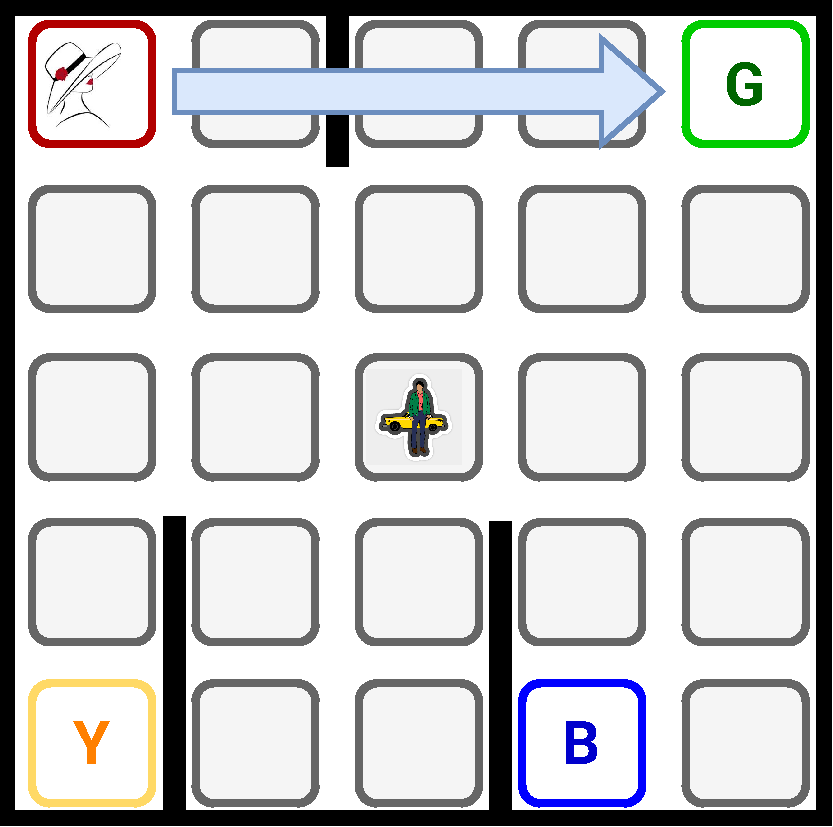
\includegraphics[scale=0.25]{Chapter5/Figs/taxi-env.pdf}
    \caption{La cuadrícula del ambiente del taxi. El taxi se encuentra en el cuadro central. El objetivo de es recoger al
    pasajero en la posición R y llevarlo a la posición G.}
    \label{fig:taxi}
\end{figure}

There are six primitive actions in this domain: (a) four navigation actions that move the taxi one square North, South, East, or West; (b) a Pickup action; and (c) a Drop off action. The six actions are deterministic.
There is a reward of -1 for each action and an additional reward of +20 for successfully
delivering the passenger. There is also a 10 point penalty for illegal pick-up and drop-off actions \cite{Dietterich:2000:HRL:1622262.1622268}.
There are 500 possible
states: 25 squares, 5 locations for the passenger (including when he's inside the cab), and 4 destinations.

\begin{figure}
    \centering
    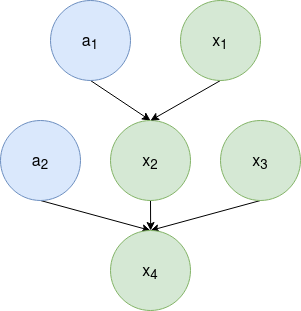
\includegraphics[scale=0.3]{Chapter5/Figs/causal_structure_taxi.png}
\end{figure}
From the model in Figure \ref{fig:cm-taxi} the color of the nodes indicates to which set of variables corresponds.
Red for actions ($A$), yellow for target variables ($Z$) and
blue for state variables ($X$). Since the environment 
is deterministic, there is no need to compute a probability 
for the value of a target variable. Instead, we evaluate whether the value of the target variable is $True$ given the action and $B$.


\subsection{Configuración experimental}

Explicar que es una tarea muy pequeña y un poco de la configuración
determinista, estocástica y lo que se compara,
cómo se mide.
También decir que aquí sólo hay dos versiones del algoritmo
y tal vez quienes son mis observaciones de alto nivel, el número
de episodio y ya. Tal vez cómo mido quién termina más rápido.
\subsection{Resultados}

\begin{figure}[H]
    \centering
    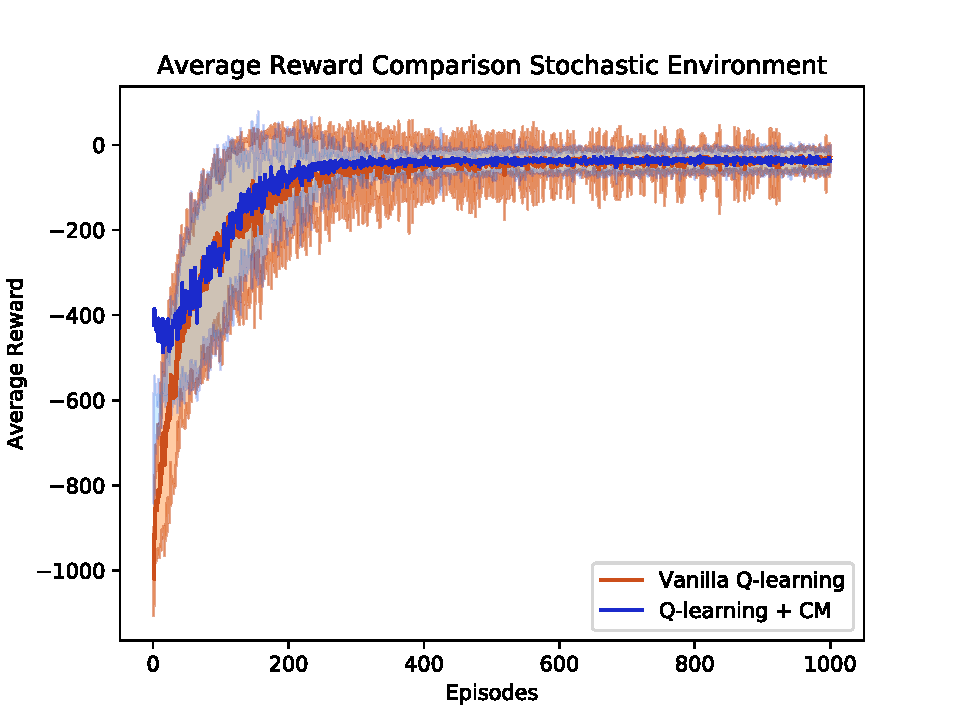
\includegraphics[scale=0.5]{Chapter5/Figs/comparisonStochastic.pdf}
\end{figure}

\section{Problema de los interruptores de luz}

\subsection{Descripción de la tarea}
Se examina la tarea de control de interruptores de luz propuesta en \cite{nair2019causal}. Un agente tiene el control
de $N$ interruptores que controlan $N$ luces en un sitio.
Cada acción $a\in \mathcal{A}$ corresponde a mover un interruptor o 
a no mover ninguno, por lo tanto $|\mathcal{A}| = N + 1$.
El agente puede percibir dos tipos de señales del ambiente,
una imagen $\mathbf{s}$ con una vista cenital del sitio, o macro-variables en forma de vectores binarios $x \in \{0,1\}^N$ que codifican las luces prendidas, donde
$x_i = 1$ si la luz en la zona $i$ está prendida, de otro modo 
toma el valor $x_i = 0$.
Para esta prueba de concepto, se trabaja con el espacio
de macro-variables $\mathcal{X}$.

Se exploran tres tipos de estructuras causales entre los
interruptores y las luces (Figura \ref{fig:struc}): \textit{uno-a-uno},
\textit{causa común} y \textit{efecto común}.

\begin{figure}[H]
    \centering
    \includegraphics[scale=0.35]{example-image-a}
    \caption{Tipos de estructuras causales}
    \label{fig:struc}
\end{figure}
La recompensa inmediata $r$ se calcula obteniendo la distancia entre
el macro-estado $x$ que observa el agente, dada la acción $a$, y la meta $g$. En este problema se usa la distancia euclidiana.

Para medir el desempeño de los algoritmos se evalúa la recompensa
promedio sobre una serie de experimentos.
Cada experimento consiste en ejecutar el algoritmo de aprendizaje durante $k$ episodios, en 
un ambiente con una estructura causal fija $\mathcal{D}$ y donde se busca alcanzar la meta $g$.
La recompensa promedio para el $i$ ésimo episodio está dada por
$R^{i} = \frac{1}{H}\sum_{t=0}^H r(s_t, a_t, g)$,
donde $H$ corresponde al tamaño del episodio.
El vector $\mathbf{R_i}$, del $i$ ésimo experimento contiene las recompensas promedio por cada episodio, y se define como
$\mathbf{R_i} = (R^{1}, \dots, R^k)$.

Finalmente, la medida de comparación entre algoritmos es
el promedio de los vectores $\mathbf{R_i}$, $i\in [1, M]$,  obtenidos en $M$ experimentos. Esta medida, denotada como  $average$ puede escribirse como 
\begin{equation}
\label{eq:average}
average(\mathbf{R_1}, \dots, \mathbf{R_M}) = \frac{1}{M}(\sum^M_i \mathbf{R_{i}^1}, \dots, \sum^M_i\mathbf{R_{i}^k}),    
\end{equation}

donde $M$ es el número de experimentos y el $\mathbf{R_i^j}$ indica la recompensa promedio obtenida en el $j$ ésimo episodio del $i$ ésimo experimento.

\subsection{Experimento 1 - Cambios en el porcentaje de completitud de $D$}

\subsubsection{Configuración experimental}

\begin{itemize}
    \item  Lorem ipsum dolor sit amet, consectetur adipiscing elit. 
    \item Duis tincidunt placerat mollis. 
    \item Curabitur a turpis varius dui iaculis maximus vel ut lectus. 
    \item Donec mollis rutrum sapien et fringilla.
    \item Sed semper risus urna, id pretium libero vulputate vel. 
    \item Vivamus eu aliquam arcu. 
    \item Vivamus ornare risus augue, a efficitur massa iaculis eu. Nullam imperdiet facilisis tellus ut ullamcorper. 
\end{itemize}
\subsubsection{Objetivo}
\subsubsection{Hipótesis del experimento}
\subsubsection{Resultados}

AMBIENTE DISCRETO

Configuración low
\begin{figure}[H]
    \centering
    \includegraphics{example-image-a}
\end{figure}


Configuración medium
\begin{figure}[H]
    \centering
    \includegraphics{example-image-b}
\end{figure}

Configuración high
\begin{figure}[H]
    \centering
    \includegraphics{example-image-c}
\end{figure}



AMBIENTE CONTINUO

Configuración low
\begin{figure}[H]
    \centering
    \includegraphics{example-image-a}
\end{figure}


Configuración medium
\begin{figure}[H]
    \centering
    \includegraphics{example-image-b}
\end{figure}

Configuración high
\begin{figure}[H]
    \centering
    \includegraphics{example-image-c}
\end{figure}


\subsection{Experimento 2 - Cambos en la tasa de consulta del modelo}



\begin{itemize}

    \item Incluir toda la información necesaria para que el estudio
    pueda ser repetido.
    \item El propósito principal del reporte es diseminar los hallazgos o resultados.
    \item Tus hallazgos deben ser descritos con mucho detalle para que el lector los juzgue.
    \item Además debe haber suficiente detalle para hacer posible
    transferir cualquier solución a algún otro lugar.
\end{itemize}    


\subsubsection{Configuración experimental}

\begin{itemize}
    \item  Lorem ipsum dolor sit amet, consectetur adipiscing elit. 
    \item Duis tincidunt placerat mollis. 
    \item Curabitur a turpis varius dui iaculis maximus vel ut lectus. 
    \item Donec mollis rutrum sapien et fringilla.
    \item Sed semper risus urna, id pretium libero vulputate vel. 
    \item Vivamus eu aliquam arcu. 
    \item Vivamus ornare risus augue, a efficitur massa iaculis eu. Nullam imperdiet facilisis tellus ut ullamcorper. 
\end{itemize}
\subsubsection{Objetivo}
\subsubsection{Hipótesis del experimento}
\subsubsection{Resultados}

AMBIENTE DISCRETO

Configuración low
\begin{figure}[H]
    \centering
    \includegraphics{example-image-a}
\end{figure}


Configuración medium
\begin{figure}[H]
    \centering
    \includegraphics{example-image-b}
\end{figure}

Configuración high
\begin{figure}[H]
    \centering
    \includegraphics{example-image-c}
\end{figure}



AMBIENTE CONTINUO

Configuración low
\begin{figure}[H]
    \centering
    \includegraphics{example-image-a}
\end{figure}


Configuración medium
\begin{figure}[H]
    \centering
    \includegraphics{example-image-b}
\end{figure}

Configuración high
\begin{figure}[H]
    \centering
    \includegraphics{example-image-c}
\end{figure}



% \subsection{Esquemas de comparación}
% \subsubsection{Q-learning}
% \subsubsection{Q-learning con estructura causal completa}
% \subsubsection{Q-learning con estructura causal incompleta}
% \subsubsection{Q-learning con estructura causal incorrecta}
% \subsection{Parámetros y medidas de desempeño}

% \section{Resultados}
% \subsection{Ambiente con estados discretos}
% \subsubsection{Experimento 1 - Cambios en el porcentaje de la completitud de $D$}
% \subsubsection{Experimento 2 - Cambios en la tasa de consulta del modelo $\epsilon$}
% \subsubsection{Experimento 3 - Transferencia de conocimiento}
% \subsection{Ambiente con estados continuos}
% \subsubsection{Experimento 1 - Cambios en el porcentaje de la completitud de $D$}
% \subsubsection{Experimento 2 - Cambios en la tasa de consulta del modelo $\epsilon$}
% \subsubsection{Experimento 3 - Transferencia de conocimiento}

% \subsection{Q-learning}
% \subsection{Q-learning con estructura causal completa}
% \subsection{Q-learning con estructura causal incompleta}
% \subsection{Q-learning con estructura causal incorrecta}


